% Hand-written text macros that depend on which results exist. Number macros inside are filled by build.sh.
\newcommand{\repoLink}{\url{https://github.com/kaiser-data/inherited-overconfidence}}
\newcommand{\llamaSummary}{A second family, Llama-3.1-8B, showed the same two audit curves but a no-audit slope of \llamaGainGZero{} (\llamaGainGZeroCI{}): there, gaps grew by about an eighth in one generation.}
\newcommand{\llamaParagraph}{We repeated the base pass, the seven teachers and the map at four audit shares on Llama-3.1-8B-Instruct (\llamaRuns{} models; base model \llamaBaseConf{}\% stated confidence, \llamaBaseAcc{}\% accuracy, gap \llamaBaseGap{}; teachers from \llamaTeacherGapMin{} to \llamaTeacherGapMax{}). The audit curves repeat: at 25, 50 and 75\% audits the greedy gain was \llamaGainGTwentyFive{}, \llamaGainGFifty{} and \llamaGainGSeventyFive{}, the sampled gain \llamaGainSTwentyFive{}, \llamaGainSFifty{} and \llamaGainSSeventyFive{} (Table~5, Appendix C). The no-audit gain differs: \llamaGainGZero{} (\llamaGainGZeroCI{}) greedy and \llamaGainSZero{} sampled, clearly above one. In this family a student was somewhat more over- or underconfident than its teacher, in both directions. \llamaChainText{}}
\newcommand{\llamaCompute}{, and about \$\llamaUsd{} for the \llamaRuns{} Llama models (A100-80GB)}
\newcommand{\llamaAppendix}{\begin{table}[h]
\centering\small
\caption{\textbf{Second family: gain by audit share for Llama-3.1-8B.} Same layout as Table~1; eight teachers.}
\tableLlama
\end{table}

\begin{figure}[h]
\centering
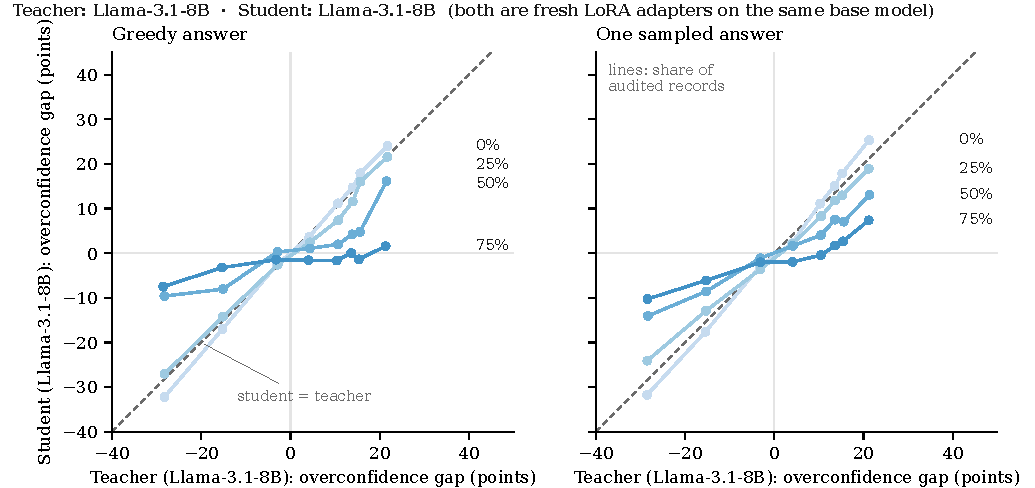
\includegraphics[width=\linewidth]{figA-return-map-llama.pdf}
\caption{\textbf{Return map for Llama-3.1-8B.} Same layout as Figure~1, four audit shares. Source: \texttt{paper/figures.py} $\to$ \texttt{results/runs\_llama31.json}.}
\end{figure}
\llamaChainTable{}}
\newcommand{\letterSummary}{worked as well (\letterAGain{}), and the tag wording alone did nothing to a model trained without tags (\probeAGain{})}
\newcommand{\letterIntro}{Two controls show the marking during training does this, not the word: a model trained without tags kept a gain of \probeAGain{} when asked under ``verified'', and meaningless tags (``K'' for audited records, ``Q'' for the rest) gave \letterAGain{} under K.}
\newcommand{\tagControls}{Two controls at 10\% separate the causes. Students trained without tags and asked under either tag kept the teacher's gap (gain \probeAGain{} and \probeBGain{}), so the word alone does nothing. Students trained with tags that have no prior meaning, ``K'' on audited records and ``Q'' on the rest, gave \letterAGain{} (\letterAGainCI{}) under K and \letterBGain{} under Q, so the meaning of ``verified'' is not needed either.}
\newcommand{\llamaChainText}{Chains for this family are reported in Appendix C if they finished before submission.}
\newcommand{\llamaChainTable}{}
